%Introduction du chapitre sur l'application : les terminaux à conteneurs

Avec le développement des échanges commerciaux qui n'ont cessé d'augmenter (de moins de 6 millions de EVP\footnote{Équivalent Vingt Pieds, en anglais \textit{TEU} : \textit{Twenty feet Equivalent Unit}. Un conteneur de 40 pieds vaut par exemple 2 EVP.} en 1970 à 500 millions de EVP en 2008)\footnote{Source : Containerization International (\url{http://www.ci-online.co.uk)}}, le conteneur est devenu la forme de conditionnement la plus répandue. Ces boîtes métalliques ont été inventées par Malcolm McLean dans les années 1930, puis normalisées d'abord par l'\textit{American National Search Institute} (anciennement l'ASA), puis par l'\textit{International Organization for Standardization} (ISO). Les dimensions principalement rencontrées sont les conteneurs de 20 et 40 pieds :
\begin{itemize}
 \item longueur : 20 pieds (6,096m) ou 40 pieds (12,192m)
 \item largeur : 8 pieds (2,438m)
 \item hauteur : 8,5 pieds (2,591m)
\end{itemize}
C'est cette normalisation qui est la cause du succès du conteneur vis-à-vis des autres modes de conditionnement. Il devient aisé de les transporter, de les manipuler et de les stocker.

\begin{figure}
 \label{fig:worldContainerTraffic}
 \begin{center}
 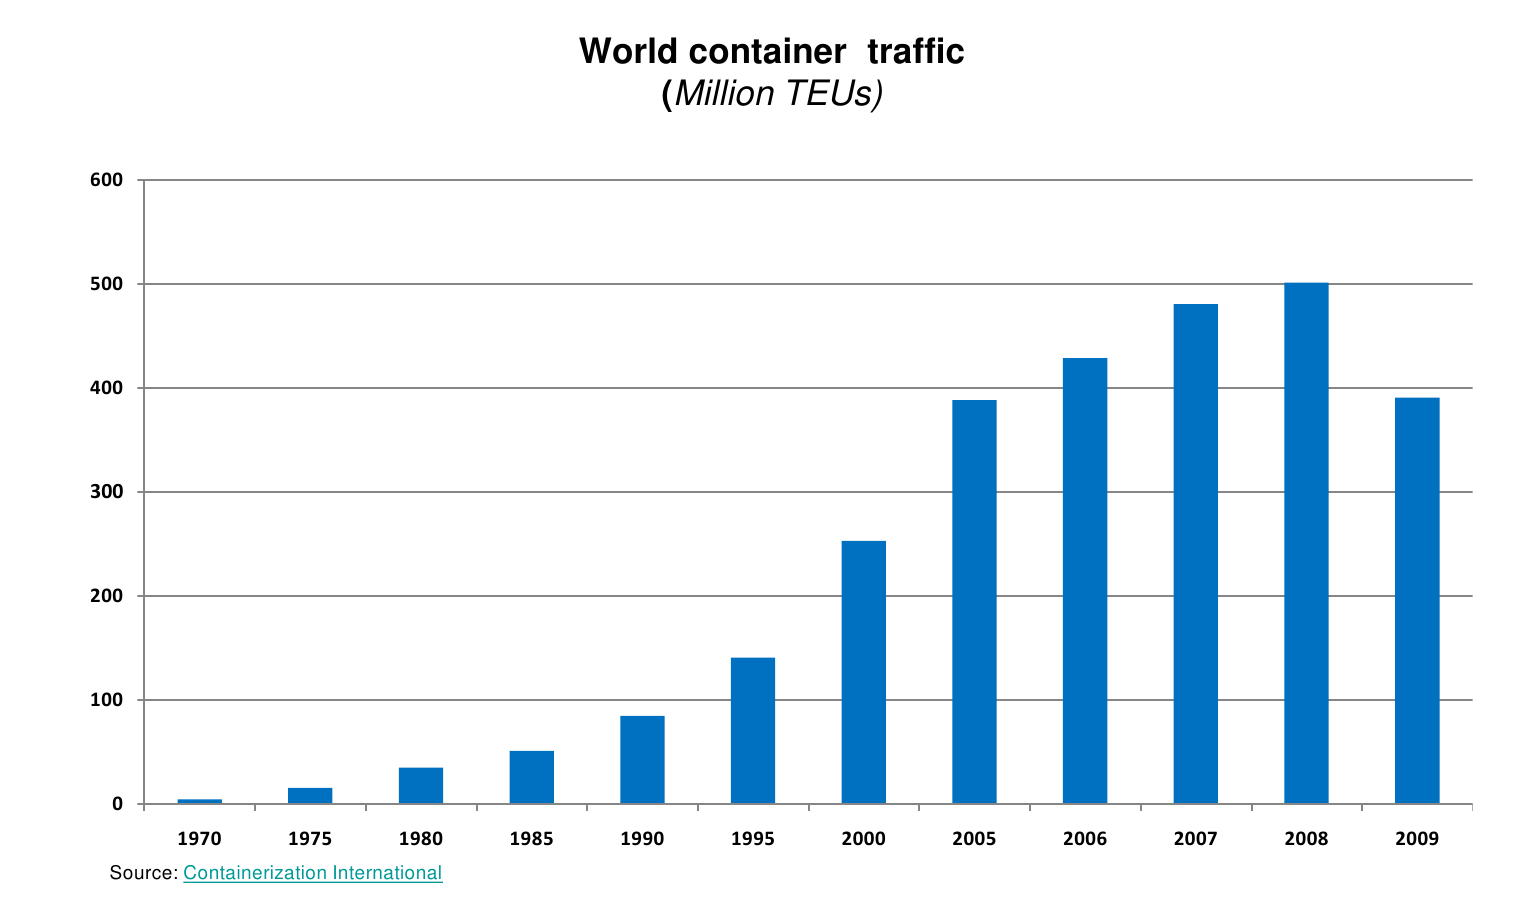
\includegraphics[width=0.75\textwidth]{chapitres/application/worldContainerTraffic.png}
 \caption{Trafic mondial de conteneurs (en millions de EVP). Source : International Transport Forum, OECD, p1.}
 \end{center}
\end{figure}

\subsection*{Identification des conteneurs}
Concernant l'identification des conteneurs, un numéro permet de les distinguer. Il s'agit d'un code décrit par la norme ISO 6346. Ce numéro est appelé numéro BIC\footnote{Bureau International des Conteneurs et du Transport Intermodal : \url{www.bic-codes.org}} et permet ainsi d'identifier de façon unique 90\% des conteneurs du trafic mondial.

\paragraph*{Structure du code BIC}
Il est composé de quatre lettres puis de six chiffres et enfin d'un dernier chiffre de contrôle permettant de vérifier qu'un numéro de série à été transmis correctement lors d'une transmission à distance. 

\begin{wrapfigure}{l}{0.28\textwidth}
 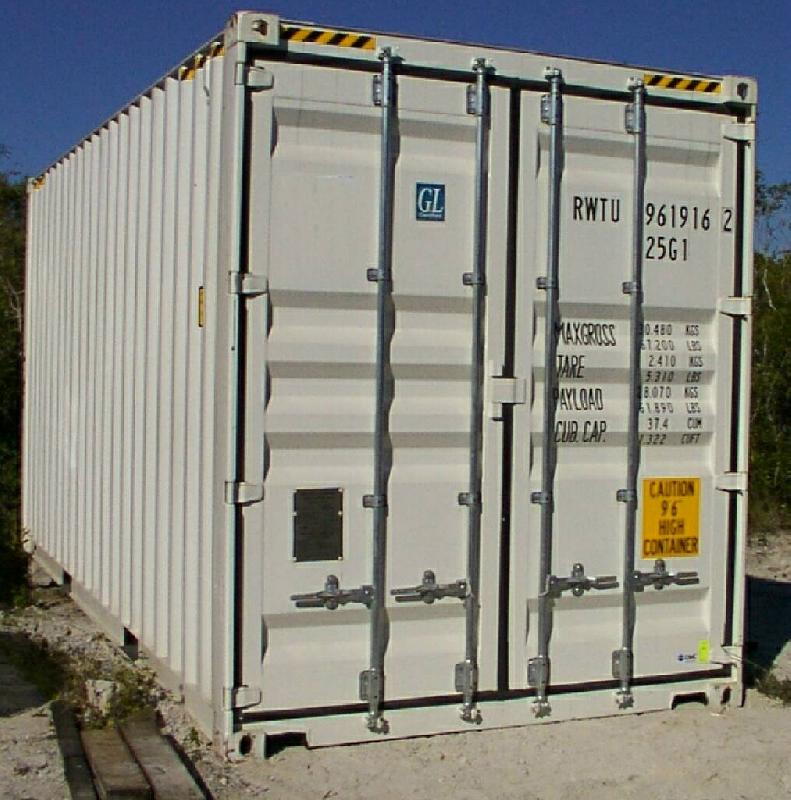
\includegraphics[width=0.28\textwidth]{chapitres/application/BICconteneur.jpg}
 \centering
 \tiny Conteneur RWTU 961916 2 
\end{wrapfigure}
Les trois premières lettres correspondent au code du propriétaire du conteneur. La quatrième lettre identifie la catégorie du conteneur : 
\begin{itemize}
 \item U : conteneur de fret;
 \item J : équipement détachable relatif à un conteneur de fret;
 \item Z : grues et châssis;
 \item R : conteneurs réfrigérés.
\end{itemize}

Les six chiffres suivants correspondent au numéro de série du conteneur. Le dernier chiffre sert de contrôle de validité du code et est calculé en 4 étapes : 

\begin{itemize}
 \item[\textbf{Étape 1 : }] un numéro est affecté à chaque lettre de l'alphabet en commençant à 10 pour la lettre A et en omettant les multiples de 11 et les chiffres de 0 à 9 conservent leur valeur : \\
 \begin{center}
 \begin{tabular}{|*{13}{p{0.5cm}|}}
  \hline
  \centering A & \centering B & \centering C & \centering D & \centering E & \centering F & \centering G & \centering H & \centering I & \centering J & \centering K & \centering L & \centering M \tabularnewline
  \hline
  \centering 10 & \centering 12 & \centering 13 & \centering 14 & \centering 15 & \centering 16 & \centering 17 & \centering 18 & \centering 19 & \centering 20 & \centering 21 & \centering 23 & \centering 24 \tabularnewline
  \hline
\end{tabular}

\huge $\text{ }$\\ %Permet d'espacer les deux tableaux
\normalsize

\begin{tabular}{|*{13}{p{0.5cm}|}}
\hline
\centering N & \centering O & \centering P & \centering Q & \centering R & \centering S & \centering T & \centering U & \centering V & \centering W & \centering X & \centering Y & \centering Z \tabularnewline
  \hline
  \centering 25 & \centering 26 & \centering 27 & \centering 28 & \centering 29 & \centering 30 & \centering 31 & \centering 32 & \centering 34 & \centering 35 & \centering 36 & \centering 37 & \centering 38 \tabularnewline
  \hline
  \end{tabular}
\end{center}

\item [\textbf{Étape 2 : }] chacun de ces nombres est multiplié par $2^{\text{indice}}$ où l'indice est la position du nombre dans le numéro BIC de gauche à droite en partant de 0.
\item [\textbf{Étape 3 : }] $\text{ }$ %Pour aller à la ligne
 \begin{itemize}
    \item[a) ] additionner tous les nombres obtenus après l'étape 2.
    \item[b) ] diviser ce résultat par 11.
    \item[c) ] supprimer la partie décimale du résultat
    \item[d) ] multiplier la partie entière ainsi obtenue par 11.
    \item[e) ] soustraire le résultat de d) du résultat de a)
   \end{itemize}
\end{itemize}

\paragraph*{Exemple : }
  \begin{itemize}
   \item[\textbf{Étape 1:}] le conteneur RWTU 961916 correspond aux valeurs suivantes : \\
   \begin{tabular}{|*{10}{p{1cm}|}}
    \hline
    \centering R & \centering W & \centering T & \centering U & \centering 9 & \centering 6 & \centering 1 & \centering 9 & \centering 1 & \centering 6\tabularnewline
    \hline
    \centering 29 & \centering 35 & \centering 31 & \centering 32 & \centering 9 & \centering 6 & \centering 1 & \centering 9 & \centering 1 & \centering 6\tabularnewline
    \hline
   \end{tabular}

   \item[\textbf{Étape 2:}] $\text{ }$\\ %Pour aller à la ligne
   \begin{tabular}{|*{10}{p{1cm}|}}
   \hline
   \centering $29*2^0$ & \centering $35*2^1$ & \centering $31*2^2$ & \centering $32*2^3$ & \centering $9*2^4$ & \centering $6*2^5$ & \centering $1*2^6$ & \centering $9*2^7$ & \centering $1*2^8$ & \centering $6*2^9$ \tabularnewline
   \hline
   \centering $29*1$ & \centering $35*2$ & \centering $31*4$ & \centering $32*8$ & \centering $9*16$ & \centering $6*32$ & \centering $1*64$ & \centering $9*128$ & \centering $1*256$ & \centering $6*512$ \tabularnewline
   \hline
   \centering 29 & \centering 70 & \centering 124 & \centering 256 & \centering 144 & \centering 192 & \centering 64 & \centering 1152 & \centering 256 & \centering 3072 \tabularnewline
   \hline
   \end{tabular}
    \item[\textbf{Étape 3:}] $\text{ }$ %Pour aller à la ligne
     \begin{itemize}
      \item[a)] $29 + 70 + 124 + 256 + 144 + 192 + 64 + 1152 + 256 + 3072 = 5359$
      \item[b)] $5349 / 11 \simeq 487.1818182$
      \item[c)] la partie entière du résultat vaut 487
      \item[d)] $487 * 11 = 5357$.
      \item[e)] $5359 - 5357 = 2$
     \end{itemize}
    \item[$\Rightarrow$] Le chiffre de contrôle de ce conteneur est donc 2.\\
  \end{itemize}


Les conteneurs sont ainsi chargés sur des navires géants appelées porte-conteneurs permettant de transporter par voie maritime des milliers de tonnes de biens aux quatre coins du monde. L'avantage majeur des conteneurs réside dans leur facilité de transbordement et c'est pourquoi un très grand nombre de plate-formes multimodales ont été créées afin de faciliter le transfert des conteneurs entre les différentes voies de transport que sont la mer, le rail et la route. Afin de réduire les durées ainsi que les coûts induits par ces transbordements, les ports doivent sans cesse innover en développant de nouvelles technologies ou en instaurant de nouveaux procédés.\\

\begin{figure}
 \begin{center}
  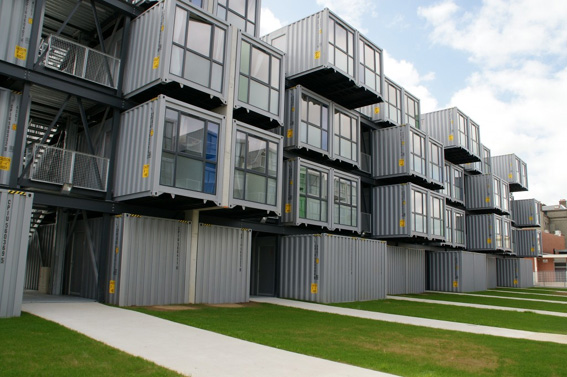
\includegraphics[width=0.65\textwidth]{chapitres/application/citeUConteneurs.jpg}
  \caption{Le succès de la conteneurisation a conduit a détourner l'utilisation principale du conteneur. Ici, la nouvelle cité universitaire du Havre.}
 \end{center}
\end{figure}

Dans ce chapitre nous détaillerons la structure et l'organisation d'un terminal portuaire à conteneurs et nous préciserons le type d'équipement présents dans ces ports. D'autre part, nous étudierons les différentes parties du terminal où une optimisation permet d'améliorer la performance de la plate-forme. Nous apporterons une attention particulière aux déplacements des conteneurs à l'intérieur du port entre les différentes zones d'échanges ainsi qu'à l'ordonnancement et à l'affectation aux véhicules des conteneurs à déplacer.